% !TEX root = ./../../_Thesis.tex

% chapter's came and label
\chapter{Introduction}
\label{chap:Introduction}

Vision is the primary channel we use to perceive the universe. Its unique capability allows us to acquire information about the surrounding world by sensing the intensity and color of light. This experience is unique and the perceived image is affected by several individual factors (\eg, refractive errors, light sensitivity, distribution of photoreceptors in the retina, etc.). Simulating visual experience is a complex and difficult task, which requires the integration of a wide range of fields, including optics, anatomy, physiology, biochemistry, psychology, and cognitive neurosciences \cite{Schwartz2010}. 

Visual aberrations can be classified as low-order or high-order. Low-order aberrations (\ie, myopia, hyperopia, astigmatism, and presbyopia) can be described in terms of sphero-cylindrical values and can be corrected with the use of eye glasses, contact lenses, or refractive surgery.  They are responsible for about 90\% of ones loss of visual acuity \cite{Dias2014}. The remaining 10\% is due to a combination of particular imperfections, known as high-order aberrations (\eg, trefoil, coma, quadrafoil, secondary astigmatism). Visual aberrations can be described by the eye's point-spread function (PSF), often represented using the so-called wavefront maps. Figure \ref{fig:eye_diagram} illustrates the human eye and the effects of some low-order aberrations when focusing at infinity. 

\begin{figure}[h]

	\centering

	\subfigure[Perfect eye]{
		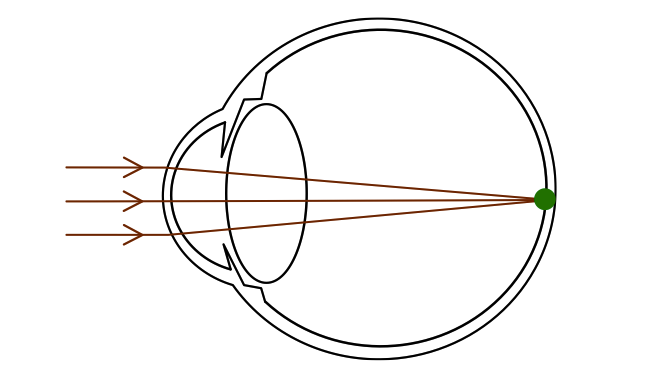
\includegraphics[width=0.28\linewidth]{__Images/01/emmetropic_eye.png}
		\label{fig:eye_diagram1}
	}
	~
	\subfigure[Myopia]{
		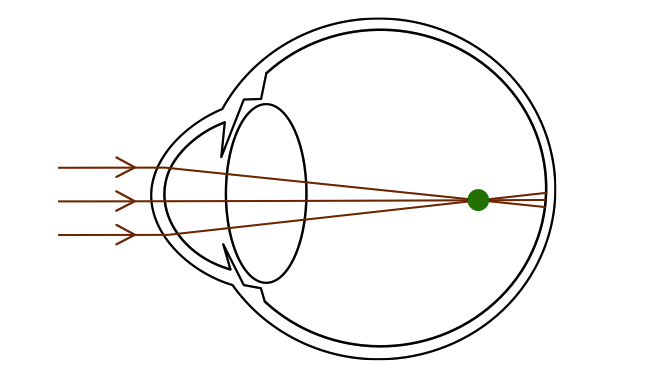
\includegraphics[width=0.28\linewidth]{__Images/01/myopic_eye.png}
		\label{fig:eye_diagram2}
	}
	~
	\subfigure[Hyperopia]{
		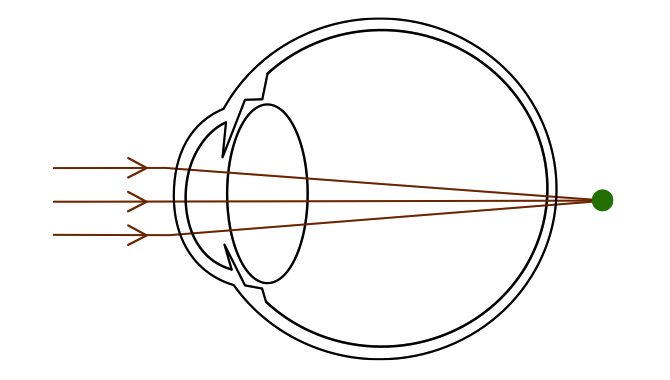
\includegraphics[width=0.28\linewidth]{__Images/01/hyperopic_eye.png}
		\label{fig:eye_diagram3}
	}

	\caption[The human eye and some low-order aberrations]{The human eye and some low-order aberrations. (a) A perfect eye focuses the parallel rays to a single point on the retina; (b) a myopic eye has an elongated eye ball or a bumped cornea, focusing parallel rays at a point before the retina; (c) a hyperopic eye has a shallow eye ball or a flatter cornea, thus focusing parallel rays at point behind the retina (modified from \cite{Pamplona2010}).}
	\label{fig:eye_diagram}
\end{figure}

The simulation of how an impaired eye perceives a scene is a complex, but highly important task. It could, for instance, give doctors an idea of how a given patient's vision was before and after some surgical procedure. It could also allow primary school teachers understand the complaints of their students. In practice, poor visual performance is often misinterpreted as the perception of blurry images. However, the problem is not that simple. Visual simulation is an intricate process that requires sophisticated tools of Fourier analysis~\cite{Thibos2011}. From a simple geometrical perspective, when the optical system of an eye is mis-focused at a point in the scene, the light emitted/reflected by such a point is spread out across some area (circle of confusion) of the retinal surface, causing blur. This can be understood from Figures \ref{fig:eye_diagram2} and \ref{fig:eye_diagram3}, and observed in Figure
%~\ref{fig:depthblur2} and 
\ref{fig:depthblur3}, which was captured using a myopic camera. Note that when the optical system is well focused (Figure \ref{fig:eye_diagram1}) a point on the scene is imaged to a point on the retina. 

Unlike traditional 2-D digital image processing in which an image is blurred by convolving it with a spatially-invariant low-pass filter kernel (Figure \ref{fig:depthblur2}), visual blurring is a depth-dependent phenomenon (\ie, the amount of blurring introduced by the eye's PSF varies with the distance from the observer's focal plane to the scene element). If depth is not taken into account by the blurring method, the resulting image might be very different from the one formed onto the retina --- Figure \ref{fig:depthblur3}.

\begin{figure}

	\centering

	\subfigure[]{
		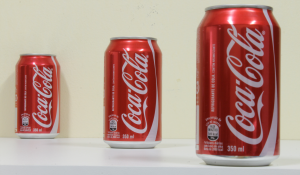
\includegraphics[width=0.75\linewidth]{__Images/01/1focused_small.png}
		\label{fig:depthblur1}
	}
	
	\subfigure[]{
		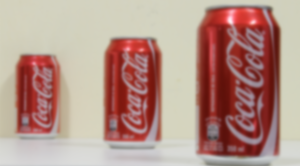
\includegraphics[width=0.75\linewidth]{__Images/01/3convolution_small.png}
		\label{fig:depthblur2}
	}
	
	\subfigure[]{
		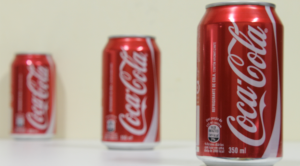
\includegraphics[width=0.75\linewidth]{__Images/01/2myopia_small.png}
		\label{fig:depthblur3}
	}

	\caption[A real scene with objects at different depths]{A real scene with objects at different depths. (a) Photograph taken with a DSLR camera, with all objects in focus; (b) result of convolving the photograph in (a) with a 2-D low-pass filter. ($\sigma$ = 15); (c) Adding an extra lens (+1 diopter) to the camera's optical system to simulate myopia. Note how the amount of blurring increases with distance. }
	\label{fig:depthblur}
\end{figure}

%\clearpage

%  Este paragrafo não pertence a este contexto
%
%\citet{Barsky2004} has explored the problem of vision simulation considering depth information and the characteristics of a particular individual's optical system. However, his technique uses synthetic scenes, since depth information is easily available for them. Moreover, Barsky's approach relies on information acquired from a high-end Shack-Hartmann wavefront sensing system (costing about USD 36,000.00). But there are plenty of other low-cost techniques to measure refractive conditions (concerning only low-order aberrations), such as the simple use of trial lenses in combination with Snellen charts, retinoscopy, auto-refractors, and others. Even though these methods do not provide the same accuracy compared with wavefront aberrometry, they are more accessible and cover most of the issues affecting people's visual acuity. 

We describe a practical approach to the simulation of visual low-order aberrations and it effects on the perception of monochromatic images placed at a known distance from the observer. The simulation is based on Fourier optics and its validation is performed using a DSLR camera.
%It relies on the assumption of a fixed depth and uses Fourier optics and a DSLR camera to simulate and validate results.

% Contributions Section
% !TEX root = ./../../_Thesis.tex

% section's Name and Label
\section{Contributions}
\label{sec:Contributions}

The \textbf{contributions} of this thesis include:

\begin{itemize}

	\item A description of a technique for modeling and simulating visual aberrations. Although the technique itself is not novel, the detailed description presented here consolidates and clarifies information from various sources, providing a valuable resource for the research community;
	\item A DLSR camera-based approach to validate the visual simulation results;
	\item The design of a psychophysical experiment to estimate an individual's absolute threshold for vision;
	\item The design and construction of an apparatus to perform the referred psychophysical experiment.
	
\end{itemize}



% Thesis Structure Section
% !TEX root = ./../../_Thesis.tex

% section's Name and Label
\section{Thesis Structure}
\label{sec:ThesisStructure}

The remaining of this thesis is organized as follows: Chapter~\ref{chap:Background} reviews the theoretical basis for the further anatomical, optical, and numerical discussions. Chapter~\ref{chap:RelatedWork} discusses previous visual simulation techniques, as well as methods for estimating optical aberrations. It also discusses simulation techniques that take non-optical characteristics into account. 
Chapter~\ref{chap:Methods} describes our approach for visual simulation of blur on monochromatic images. 
%Additionally, it explains how the technique can be combined with the minimum amount of light perceived by an individual. 
Chapter~\ref{chap:Results} presents a study about the absolute threshold for vision and an attempt to relate it with the spherical equivalent refraction. 
Finally, Chapter~\ref{chap:Discussion} summarizes this thesis and suggests some ideas for future work.

%focused on statistically significant data and their limitations.

%summarizes this thesis and suggests some ideas for future work.

% removi
% , discusses statistically significant data and their limitations,

% XYZ Section
% \input{__Text/01_Introduction/130.tex}

% XYZ Section
% \input{__Text/01_Introduction/140.tex}

% XYZ Section
% \input{__Text/01_Introduction/150.tex}